\subsubsection*{ -- Electrical}\par

The electrical design plays a major role in the design of the system, which ranges from the NI myRIO device itself to the sensing and actuating systems, and finally the noise filtering methods. Connected to the myRIO are 3 electrical systems that are very crucial to the project namely: the encoder, load cell, and the motor and its amplifier shown in Figure \ref{Wiring_Toon}.\par
\begin{figure}[htbp]
\begin{center}
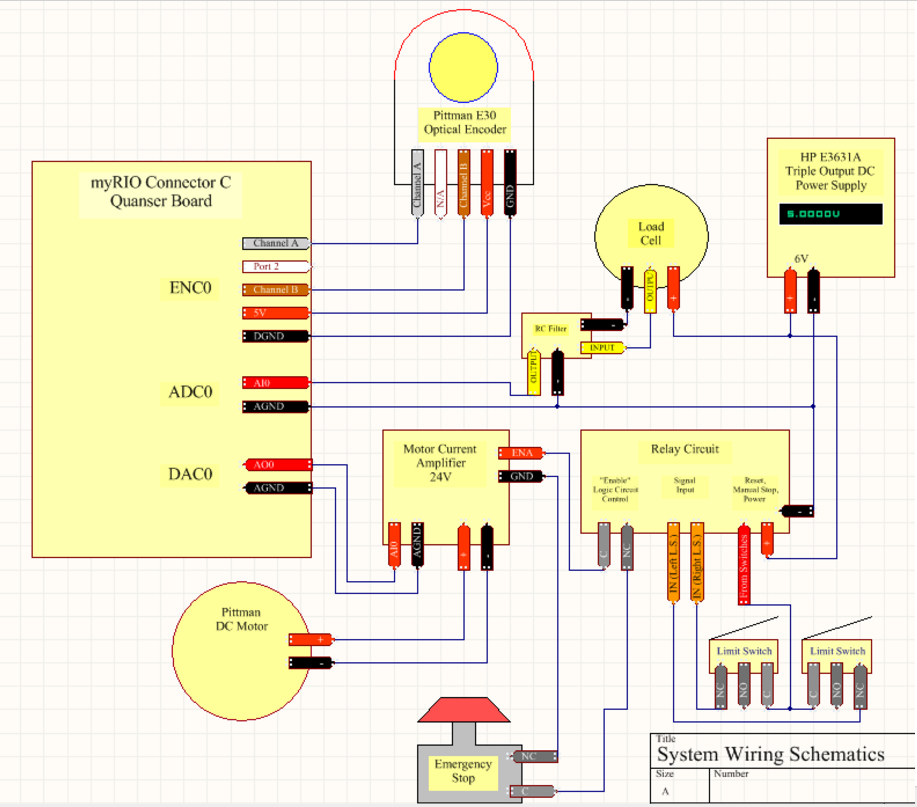
\includegraphics[width=2.75in]{Images/Cartoon_Electrical.PNG}
\caption{System Wiring Overview}
\label{Wiring_Toon}
\end{center}
\end{figure}
\vspace{.167in}
\noindent\underline{NI myRIO-1900} \par
\vspace{.08in}
National Instruments myRIO-1900 is a reconfigurable I/O device with a dual-core ARM Cortex A9 chip and a Xilinx FPGA customizable I/O. Using a Field-Programmable Gate Arrays (FPGAs) allows the chip to rewire itself every time a new program is inserted, which allows for faster implementation and testing of the controller C code. Additionally, myRIO have built-in Digital-to-Analog Converters (DAC) and Analog-to-Digital Converters (ADC) providing analog inputs (AI) and outputs (AO) as well as digital inputs and outputs (DIO).\par In the case of this project, the I/O is connected to the motor and sensors through a quanser board that is connected to the connector-c of the myRIO. A LCD display and keypad for user interaction is also connected to the I/O, but through connector-b of the myRIO.\par
\vspace{.167in}
\noindent\underline{Pittman DC040B-5 Motor}\par
\vspace{.08in}
The Pittman motor is a 24V brush DC motor with a gearing of 5.9:1 and it also includes an encoder at the back of the motor. The motor was chosen based on the requirements shown in Table 1, which are derived from the simulation results as shown in the Analysis section above. \par
The motor is connected to a 24V motor amplifier, which is then connected to the DAC in the myRIO through the quanser board using a BNC connector.\par
For added safety during operation, limit switches are added to both ends of the track. When the either of the switches are depressed, it activates a relay circuit which will open an ``ENABLE'' logic circuit in the amplifier and cuts off power to the motor as well as lighting up a red LED. There is also a switch-box where the operator could press a green ``Reset'' button to open the relay circuit and allow the motor to run again, a red ``Stop'' button for activating the relay circuit on demand, and an emergency switch which would immediately open the ``ENABLE'' logic circuit if the neither the relay circuit nor its power supply is working.\par

\begin{table}[]
\centering
\caption{Simulation Summary for Motor Requirements}
\label{Table 1}
\begin{tabular}{|l|c|c|}
\hline
                       & \textbf{Simulated Results} & \textbf{Actual Specs.} \\ \hline
\textbf{Rated Toque}   & 0.2Nm                      & 0.4Nm                  \\ \hline
\textbf{Rated Current} & 0.6A                       & 1.82A                  \\ \hline
\textbf{Max. Voltage}  & 24.5V                      & 24V                    \\ \hline
\textbf{Max. Torque}   & 2Nm                        & 2.6Nm                  \\ \hline
\textbf{Max. Current}  & 5.8A                       & 9.64A                  \\ \hline
\textbf{Gear Ratio}    & 5.9                        & 5.9                    \\ \hline
\end{tabular}
\end{table}

\vspace{.167in}
\noindent\underline{E30 Pittman Optical Encoder}\par
\vspace{.08in}
The encoder included in the motor have 512 slots, and with quadrature encoding it gives us 2048 pulses/revolution allowing the controller to get an accurate position data. The wires coming out of the encoder are soldered onto a DIN cable so as to be able to plug it into the ENC0 port of the myRIO quanser board.\par 
\vspace{.167in}
\noindent\underline{FC22 Compression Load Cell}\par
\vspace{.08in}
The FC22 compression load cell sensor is used to detect the force input. It has a range to detect 0-50lbf or 0-22.68kg giving a range of 0-226.8N which is more than the required range. This particular load cell is also chosen because of its small form factor, as it also includes its own amplifier within a small package. It is supplied by a 5V power supply, and gives an output signal of 0.5-4.5V. \par
Even though it can be assumed that the relation between the voltage output and the force input is linear, calibration was still performed using known mass and finding its corresponding voltage outputs. The data points are then plotted, and the coefficients of the linear line are implemented in the C code converting between voltage input to force input for the controller. \par
In order to allow bi-directional detection of forces, the load cell is pre-loaded using the M10 bolt to a midpoint of 2.5V. Thus, if the load cell is pre-loaded to the right, and the controller sees an increase in voltage it knows that the force is acting to the right (compressing it). If the voltage decreases, then the force is acting to the left (de-compressing it).The output is then connected to a capacitor and then to the myRIO quanser board ADC0 port. \par
\vspace{.167in}
\noindent\underline{Noise and Filtering}\par
\vspace{.08in}
\begin{figure}[ht]
\begin{center}
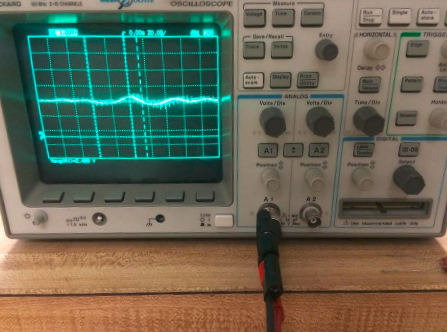
\includegraphics[width=2.75in]{Images/Before_Filter.PNG}
\caption{Noise observed before filtering}
\label{B_Filter}
\end{center}
\end{figure}
\begin{figure}[ht]
\begin{center}
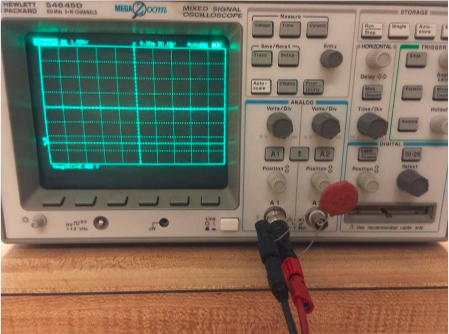
\includegraphics[width=2.75in]{Images/After_Filter.PNG}
\caption{Minimal noise observed after Filtering}
\label{A_Filter}
\end{center}
\end{figure}
As seen from Figure \ref{B_Filter} and \ref{A_Filter}, the load cell output can be noisy and it will make the controller thinks that a force is a applied to the cart when there is none. To filter out the noise, the load cell output is first connected to a 0.1$\mu$F capacitor before going into the myRIO quanser board. This equals to using an RC Filter as the output impedance of the load cell amplifier acts a resistance (R) and the capacitor is the capacitance (C). And in the C code itself, a 1N deadband is also implemented to allow the controller to ignore any force input that is smaller than 1N further reduce the sensitivity of the controller to the noise.
